% E.15 △ABC, ∠BAC=90°, AB=AC. △ABD 绕 A 顺时针 90° → △ACE.
% A(0,0), B(0,7.07), C(7.07,0) (AB=AC=10/√2·... 取 AB=AC=10/√2 让 BC=10? BC=AB√2 = 10 → AB=AC=5√2 ≈7.07)
% 简化: 取 AB=AC=7. D 在 BC 上. BD=3, CD=4. BC=7 (不是7√2)? 用题(2): BC=AB√2. 若 BD=3,CD=4,BC=7 → AB=7/√2.
% 用题(2)情形: BC=7, AB=AC=7/√2≈4.95. A(0,0), B(0,7/√2), C(7/√2,0).
% D 在 BC: B+3/7·(C-B). C-B=(7/√2, -7/√2). D = (3/√2, 7/√2-3/√2) = (3/√2, 4/√2) ≈ (2.121, 2.828)
% E = D 绕 A 顺时针 90°: (x,y)→(y,-x) → E=(4/√2, -3/√2) ≈ (2.828, -2.121)
\documentclass[tikz,border=4pt]{standalone}
\usepackage{ctex}
\usepackage{amsmath}
\usetikzlibrary{calc}
\begin{document}
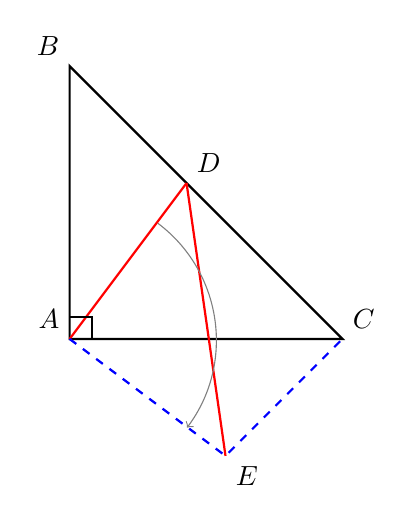
\begin{tikzpicture}[scale=0.7, thick]
  \coordinate (A) at (0,0);
  \coordinate (B) at (0,4.9497);
  \coordinate (C) at (4.9497,0);
  \coordinate (D) at (2.1213, 2.8284);
  \coordinate (E) at (2.8284, -2.1213);

  \draw (A)--(B)--(C)--cycle;
  \draw[red, thick] (A)--(D);
  \draw[blue, dashed, thick] (A)--(E)--(C);
  \draw[red, thick] (D)--(E);

  % 直角 ∠A
  \draw (0.4,0)--(0.4,0.4)--(0,0.4);

  % 旋转弧
  \draw[->, gray, thin] (1.6,2.1) arc[start angle=53.13, end angle=-36.87, radius=2.65];

  \node[above left] at (A) {$A$};
  \node[above left] at (B) {$B$};
  \node[above right] at (C) {$C$};
  \node[above right] at (D) {$D$};
  \node[below right] at (E) {$E$};
\end{tikzpicture}
\end{document}
